\documentclass{article}
\usepackage{amsmath}
\usepackage{amsthm}
\usepackage{amssymb}
\usepackage{enumitem}
\usepackage{tikz}
\usepackage{tikz-qtree}
\usepackage{tikz-qtree-compat}
\usetikzlibrary{positioning}
\usetikzlibrary{trees}
%\usepackage[paperheight=29.7cm,paperwidth=21cm,margin=1cm]{geometry}

\title{Answers for Chapter 2: A SIMPLE SYNTAX-DIRECTED TRANSLATOR}
\author{hmsjwzb@zoho.com}
\date{\today}

\begin{document}
	
\maketitle
\newpage
\section*{2.2.7 Exercises for Section 2.2}

\textbf{Exercise 2.2.1 :} Consider the context-free grammar
\[
S \rightarrow S\, S + \mid S\, S\, * \mid a
\]

\begin{enumerate}[label=\alph*)]
	\item Show how the string \(aa+a*\) can be generated by this grammar
	\item Construct a parse tree for this string
	\item What language does this grammar generate? Justify your answer.
\end{enumerate}

\textbf{Answer:}
\begin{enumerate}[label=\textbf{\alph*)}]
	\item Apply the following production in sequence.
	\begin{align*}
		&S \rightarrow S_1\,S_2\,*\\
		&S_1 \rightarrow S_3\,S_4\,+\\
		&S_3 \rightarrow a\\
		&S_4 \rightarrow a\\
		&S_2 \rightarrow a
	\end{align*}

	\item The parse tree for it
	\begin{center}
		\begin{tikzpicture}[
			grow=south,
			level 1/.style={sibling distance=20mm},
			level 2/.style={sibling distance=10mm},
			level distance=15mm,
			every node/.style={circle, minimum size=5mm},
			]
			\node {S}
			child { node {S} 
				child { node {S} child{node {a}}}
				child { node {S} child{node {a}}}
				child { node {+} }
			}
			child { node {S} 
				child { node {a} }
			}
			child { node {*}
			};
		\end{tikzpicture}
	\end{center}

	\item This language generate post-fix expression with + and * as operator, a as operand
\end{enumerate}
\newpage

\textbf{Exercise 2.2.2:} What language is generated by the following grammars? In each case justify your answer.
\begin{enumerate}[label=\textbf{\alph*)}]
	\item $S \to 0\ S\ 1 \mid 0\ 1$
	\item $S \to +\ SS \mid -\ SS \mid a$
	\item $S \to S\ (\ S\ )\ S \mid \epsilon$
	\item $S \to a\ S\ b\ S \mid b\ S\ a\ S \mid \epsilon$
	\item $S \to a \mid S\ +\ S \mid S\ S \mid S\ * \mid (\ S\ )$
	%\item $S\,\rightarrow\,0\,S\,1\,|\,0\,1$
	%\item $S\,\rightarrow \,+\, S\, S\, |\, -\, S\, S\, |\, a$
\end{enumerate}
\textbf{Answer:}
\begin{enumerate}[label=\textbf{\alph*)}]
	\item A language contain first half as 0, second half as 1
	\item A pre-fix expression with + and - as operator and a as operator
	\item matched Parentheses
	\item A language with same number of a and b
	\item An infix expression with + and * as operator and a as operand
\end{enumerate}

\newpage
\textbf{Exercise 2.2.3:} Which of the grammars in Exercise 2.2.2 are ambiguous?
\textbf{Answer:}
\begin{enumerate}[label=\textbf{\alph*)},start=3]
	\item $S \to S\ (\ S\ )\ S \mid \epsilon$ is ambiguous, the input ()() has two corresponding grammar tree.
	\begin{center}
		\begin{figure}[htbp]
			\begin{tikzpicture}[level distance=1cm, sibling distance=1.2cm]
				\Tree [.S 
				[.S $\epsilon$ ]
				[.( ( ]
				[.S $\epsilon$ ]
				[.) ) ]
				[.S 
				[.S $\epsilon$ ]
				[.( ( ]
				[.S $\epsilon$ ]
				[.) ) ]
				[.S $\epsilon$ ]
				]
				]
			\end{tikzpicture}
			\caption{grammar tree 1}
		\end{figure}
		\begin{figure}[htbp]
			\begin{tikzpicture}[level distance=1cm, sibling distance=1.2cm]
				\Tree [.S 
				[.S 
				[.S $\epsilon$ ]
				[.( ( ]
				[.S $\epsilon$ ]
				[.) ) ]
				[.S $\epsilon$ ]
				]
				[.( ( ]
				[.S $\epsilon$ ]
				[.) ) ]
				[.S $\epsilon$ ]
				]
			\end{tikzpicture}
			\caption{grammar tree 2}
		\end{figure}
	\end{center}
	\newpage
	\item $S \to a\ S\ b\ S \mid b\ S\ a\ S \mid \epsilon$ is ambiguous
	\begin{center}
	\begin{figure}[htbp]
		\begin{tikzpicture}[level distance=1.5cm, sibling distance=1.5cm]
			\node {S}
			child { node {a} }
			child { node {S}
				child { node {\(\epsilon\)} }
			}
			child { node {b} }
			child { node {S}
				child { node {a} }
				child { node {S}
					child { node {\(\epsilon\)} }
				}
				child { node {b} }
				child { node {S}
					child { node {\(\epsilon\)} }
				}
			};
	\end{tikzpicture}
	\caption{ Derivation for abab}
	\end{figure}
	\begin{figure}[htbp]
		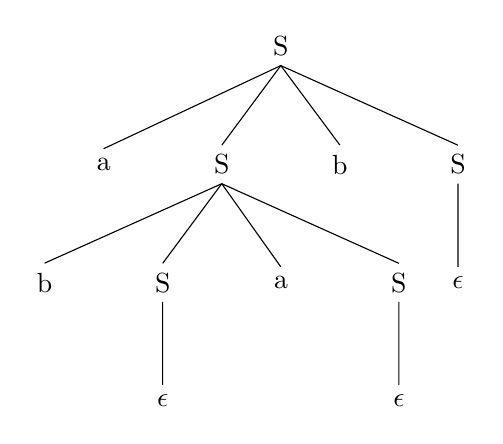
\begin{tikzpicture}[level distance=1.5cm, sibling distance=1.5cm]
		\node {S}
			child { node {a} }
			child { node {S} 
					child { node{b} }
					child { node{S}
							child { node {\(\epsilon\)} }}
					child { node{a} }
					child { node{S} 
							child { node {\(\epsilon\)} }}
					}
			child { node {b} }
			child { node {S} 
					child { node {\(\epsilon\)} }};
		\end{tikzpicture}
		\caption{ Derivation for abab}
	\end{figure}
\end{center}
\end{enumerate}
\newpage
\textbf{Exercise 2.2.4:} Construct unambiguous context-free grammars for each of the following languages. In each case show that your grammar is correct.
\begin{enumerate}[label=\textbf{\alph*)}]
	\item Arithmetic expressions in postfix notation.
	\item Left-associative lists of identifiers separated by commas.
	\item Right-associative lists of identifiers separated by commas.
	\item Arithmetic expressions of integers and identifiers with the four binary operators +,-,*,/.
	\item[\textbf{!e)}] Add unary plus and minus to arithmetic operators of (d)
\end{enumerate}
\textbf{Answer:}
\begin{enumerate}[label=\textbf{\alph*)}]
	\item Arithmetic expressions in postfix notation.
	\begin{align*}
		expr &\rightarrow expr\ expr\ operator\\
			 &\hspace*{13pt}|\ operand\ operand\ operator\\
		operator &\rightarrow +\ -\ *\ \div\\
		operand &\rightarrow [1-9]\ remain\\
		remain &\rightarrow [0-9]\ remain\\
	\end{align*}

	\item Left-associative lists of identifiers separated by commas.
	\begin{align*}
		list\ &\rightarrow list,\ \mathtt{ident}
	\end{align*}
	
	\item Right-associative lists of identifiers separated by commas.
	\begin{align*}
		list\ &\rightarrow \mathtt{ident},\ list
	\end{align*}

	\item Arithmetic expressions of integers and identifiers with four binary operator $+, -, *, /$
	\begin{align*}
		expr\ &\rightarrow\ expr\ operand\ integer\\
			\ &\hspace{12pt}|\ integer\\
		operand\ &\rightarrow\ \mathtt{+}\ |\  \mathtt{-}\ |\ \mathtt{*}\ |\ \ \mathtt{/}\\
		integer\ &\rightarrow\ msd\  remain\\
		msd\ &\rightarrow\ [1..9]\\
		remain\ &\rightarrowtail\ [0..9]^*\ remain
	\end{align*}
\newpage
	\item[\textbf{!e)}] Add unary plus and minus arithmetic operators of (d)
	\begin{align*}
		expr\ &\rightarrow\ expr\ operand\ unary\\
		\ &\hspace{12pt}|\ unary\\
		unary &\rightarrow\ -\ integer\\
		&\hspace{12pt}|\ +\ integer\\
		operand\ &\rightarrow\ \mathtt{+}\ |\  \mathtt{-}\ |\ \mathtt{*}\ |\ \ \mathtt{/}\\
		integer\ &\rightarrow\ msd\  remain\\
		msd\ &\rightarrow\ [1..9]\\
		remain\ &\rightarrowtail\ [0..9]^*\ remain
	\end{align*}
\end{enumerate}
\textbf{Exercise 2.2.5:}
\begin{enumerate}[label=\textbf{\alph*)}]
	\item Show that all binary strings generated by the following grammar have values divisible by 3. \textit{Hint.} Use induction on the number of nodes in parse tree.
	\begin{align*}
		num\ \rightarrow\ 11\ |\ 1001\ |\ num\ 0\ |\ num\ num
	\end{align*}
	\item Does the grammar generate all binary strings with values divisible by 3?
\end{enumerate}

\begin{enumerate}[label=\textbf{\alph*)}]
	\item Show that all binary strings generated by the following grammar have values divisible by 3. \textit{Hint.} Use induction on the number of nodes in parse tree.
	\begin{align*}
		num\ \rightarrow\ 11\ |\ 1001\ |\ num\ 0\ |\ num\ num
	\end{align*}
	\begin{enumerate}
		\item The binary strings are divisible by 3
		\begin{proof}
			\[num\ \rightarrow\ 11\ | \ 1001 \] 
			The show terminal symbol generated by num are divisible by 3.\\
			A sum of every digit of a number is divisible 3, then the number is divisible by 3.
	
	\begin{minipage}{0.45\textwidth}
		\centering
		\begin{tikzpicture}[
			every node/.style={minimum width=2cm, minimum height=1cm, align=center},
			sibling distance=2cm,
			level distance=1.5cm
			]
			\node {num}
			child { node {num} }
			child { node {0} };
		\end{tikzpicture}
	\end{minipage}\hfill
	\begin{minipage}{0.45\textwidth}
		\centering
		\begin{tikzpicture}[
			every node/.style={minimum width=2cm, minimum height=1cm, align=center},
			sibling distance=2cm,
			level distance=1.5cm
			]
			\node {num}
			child { node {num} }
			child { node {num} };
		\end{tikzpicture}
	\end{minipage}
	\newline
		As we can see from above grammar tree, the sum of all digits of num is divisible by 3.
		So it should be divisible by 3.
		\end{proof}
	\newpage
	\item Does the grammar generate all binary strings with values divisible by 3?\newline
	Yes, it generate all binary strings with values divisible by 3.
	\end{enumerate}
\end{enumerate}
\textbf{Exercise 2.2.6:}
Construct a context-free grammar for roman numerals
\begin{enumerate}[label=\textbullet]
	\item via wikipedia, we can categorize the single roman numerals into 4 groups:
	\begin{align*}
		I,\ II,\ III\ |\ I\ V\ |\ V,\ V\ I,\ V\ II,\ V\ III\ |\ I\ X
	\end{align*}
	then get the production:
	\begin{align*}
		&digit\ \rightarrow\ smallDigit\ |\ I\ V\ |\ V\ smallDigit\ |\ I\ X\\
		&smallDigit\ \rightarrow\ I\ |\ II\ |\ III\ | \epsilon
	\end{align*}
	
	\item find a simple way to map roman to arabic numerals. For example
	\begin{enumerate}
		\item $XII => X,\ II => 10 + 2 => 12$
		\item $CXCIX => C,XC,IX => 100 + 90 + 9 => 199$
		\item $MDCCCLXXX => M, DCCC, LXXX => 1000 + 800 + 80 => 1880$
	\end{enumerate}
	
	\item via the upper two rules, derive the production
	\begin{align*}
	romanNum\ &\rightarrow\ thround\ hundred\ ten\ digit\\
	throusand\ &\rightarrow\ M\ |\ MM\ |\ MMM\ |\ \epsilon\\
	hundred\ &\rightarrow\ smallHundred\ |\ C\ D\ |\ D\ smallHundred\ |\ C\ M\\
	smallHundred\ &\rightarrow\ C\ |\ CC\ |\ CCC\ |\ \epsilon\\
	ten\ &\rightarrow\ smallTen\ |\ X\ L\ |\ L\ smallTen\ |\ X\ C\\
	smallTen\ &\rightarrow\ X\ |\ XX\ |\ XXX\ |\ \epsilon\\
	digit\ &\rightarrow\ smallDight\ |\ I\ V\ |\ V\ smallDigit\ |\ I\ X\\
	smallDigit\ &\rightarrow\ I\ |\ II\ |\ III\ |\ \epsilon
	\end{align*}
\end{enumerate}
\end{document}